\documentclass[a4paper,11pt]{article}
\usepackage{amsmath,amsthm,amsfonts,amssymb,amscd,amstext,vmargin,graphics,graphicx,tabularx,multicol} \usepackage[french]{babel}
\usepackage[utf8]{inputenc}  
\usepackage[T1]{fontenc} 
\usepackage[T1]{fontenc}
\usepackage{amsmath,amssymb}
\usepackage{pstricks-add,tikz,tkz-tab,variations}
\usepackage[autolanguage,np]{numprint} 
\usepackage{color}
\usepackage{ulem}

\setmarginsrb{1.5cm}{0.5cm}{1cm}{0.5cm}{0cm}{0cm}{0cm}{0cm} %Gauche, haut, droite, haut
\newcounter{numexo}
\newcommand{\exo}[1]{\stepcounter{numexo}\noindent{\bf Exercice~\thenumexo} : \marginpar{\hfill /#1}}
\reversemarginpar


\newcounter{enumtabi}
\newcounter{enumtaba}
\newcommand{\q}{\stepcounter{enumtabi} \theenumtabi.  }
\newcommand{\qa}{\stepcounter{enumtaba} (\alph{enumtaba}) }
\newcommand{\initq}{\setcounter{enumtabi}{0}}
\newcommand{\initqa}{\setcounter{enumtaba}{0}}

\newcommand{\be}{\begin{enumerate}}
\newcommand{\ee}{\end{enumerate}}
\newcommand{\bi}{\begin{itemize}}
\newcommand{\ei}{\end{itemize}}
\newcommand{\bp}{\begin{pspicture*}}
\newcommand{\ep}{\end{pspicture*}}
\newcommand{\bt}{\begin{tabular}}
\newcommand{\et}{\end{tabular}}
\renewcommand{\tabularxcolumn}[1]{>{\centering}m{#1}} %(colonne m{} centrée, au lieu de p par défault) 
\newcommand{\tnl}{\tabularnewline}

\newcommand{\trait}{\noindent \rule{\linewidth}{0.2mm}}
\newcommand{\hs}[1]{\hspace{#1}}
\newcommand{\vs}[1]{\vspace{#1}}

\newcommand{\N}{\mathbb{N}}
\newcommand{\Z}{\mathbb{Z}}
\newcommand{\R}{\mathbb{R}}
\newcommand{\C}{\mathbb{C}}
\newcommand{\Dcal}{\mathcal{D}}
\newcommand{\Ccal}{\mathcal{C}}
\newcommand{\mc}{\mathcal}

\newcommand{\vect}[1]{\overrightarrow{#1}}
\newcommand{\ds}{\displaystyle}
\newcommand{\eq}{\quad \Leftrightarrow \quad}
\newcommand{\vecti}{\vec{\imath}}
\newcommand{\vectj}{\vec{\jmath}}
\newcommand{\Oij}{(O;\vec{\imath}, \vec{\jmath})}
\newcommand{\OIJ}{(O;I,J)}

\newcommand{\bmul}[1]{\begin{multicols}{#1}}
\newcommand{\emul}{\end{multicols}}


\newcommand{\reponse}[1][1]{%
\multido{}{#1}{\makebox[\linewidth]{\rule[0pt]{0pt}{20pt}\dotfill}
}}

\newcommand{\titre}[5] 
% #1: titre #2: haut gauche #3: bas gauche #4: haut droite #5: bas droite
{
\noindent #2 \hfill #4 \\
#3 \hfill #5

\vspace{-1.6cm}

\begin{center}\rule{6cm}{0.5mm}\end{center}
\vspace{0.2cm}
\begin{center}{\large{\textbf{#1}}}\end{center}
\begin{center}\rule{6cm}{0.5mm}\end{center}
}



\begin{document}
\pagestyle{empty}
\titre{Contrôle 1 : Théorème de Pythagore, de Thalès et les statistiques }{Nom}{Prénom}{Date}{Classe}

\begin{flushleft}
\begin{tabular}{|m{9.5cm}|m{1.25cm}|m{1.25cm}|m{1.25cm}|m{1.25cm}|m{1.25cm}|}
\hline 
\textbf{Compétences} & \begin{center}
\textbf{N.E.}
\end{center} & \begin{center}
\textbf{M.I.}
\end{center} & \begin{center}
\textbf{M.F.}
\end{center}  & \begin{center}
\textbf{M.S.}
\end{center} & \begin{center}
\textbf{T.B.M.}
\end{center} \\ 
\hline 
Je dois savoir traduire en langage mathématique une situation réelle &  &  & & &\\
\hline 
Je dois savoir extraire d'un document les informations utiles, les reformuler, les organiser, les confronter à mes connaissances &  &  & & &\\
\hline
\end{tabular} 
\end{flushleft}

\textit{N.E = Non évalué ; M.I. = Maîtrise insuffisante ; M.F. = Maîtrise fragile ; M.S. = Maîtrise satisfaisante ; T.B.M. = Très bonne maîtrise}\\


\vspace*{0.5cm}

\exo{6}


\bmul{2}

A partir des information portées sur le dessin suivant, démontrer que les droites (EF) et (FG) sont perpendiculaires.

\columnbreak

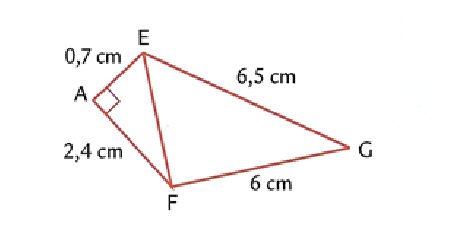
\includegraphics[scale=1.1]{difficicel.eps} 


\emul


\exo{3} La figure n'est pas faite en vraie grandeur.	
\bmul{2}			    
	
Pour la figure ci-contre, on sait que :	\\
- Les droites (BC) et (DF) sont parallèles, 	\\			       
- AC = 18 cm ;  CG = 9 cm ;  GE = 15 cm  et  EF = 22,5 cm.		\\

\initq \q	Vérifier que : BC = 13,5 cm.\\

\columnbreak


\includegraphics[scale=0.7]{thales.eps} 

\emul

\exo{3} Dans un coin de sa chambre mansardée, Lucie installe une étagère comme représentée sur le schéma ci-dessous. \\
Lucie a l'impression que son étagère n'est pas droite (c'est-à-dire non parallèle au sol). A-t-elle raison ?
\begin{center}

\includegraphics[scale=0.7]{recithales.eps} 
\end{center}

\newpage

\vspace*{0.5cm}

\exo{5.5} Un professeur de SVT demande aux 29 élèves d'une classe de sixième de faire germer des graines de blé chez eux.\\

Le professeur donne un protocole expérimental à suivre.
\bi
\item Mettre en culture sur du coton dans une boîte placée dans une pièce éclairée, de température entre \\
20 \degre C et 25\degre C.
\item Arroser une fois par jour.
\item Il est possible de couvrir les graines avec un film transparent pour éviter l'évaporation de l'eau.\\
\ei

Le tableau ci-dessous donne les tailles des plantules (petites plantes) des 29 élèves à 10 jours après la mise en germination.\\


\renewcommand{\arraystretch}{1.8}

\begin{tabular}{|c|c|c|c|c|c|c|c|c|c|c|c|}
\hline 
Taille (en cm) & 0 & 8 & 12 & 14 & 16 & 17 & 18 & 19 & 20 & 21 & 22 \\ 
\hline 
Effectifs & 1 & 2 & 2 & 4 & 2 & 2 & 3 & 3 & 4 & 4 & 2 \\ 
\hline 
\end{tabular} 

\vspace*{0.4cm}

\initq \q  Combien de plantules ont une taille qui mesure au plus 12 cm ?\\

\q Donner les valeurs extrêmes de cette série.\\

\q Calculer la moyenne de cette série. Arrondir au dixième près.\\

\q Quel pourcentage des élèves de la classe a obtenu une plantule qui mesure au plus 18 cm ?\\


\q On considère qu'un élève a bien respecté le protocole si la taille de la plantule à 10 jours est supérieure ou égale à 14 cm.\\
Quel pourcentage des élèves de la classe a bien respecté le protocole ?\\

\vspace*{0.5cm}

\exo{2.5}
On s'intéresse à une course réalisée au début de l'année 2018. \\
Il y a 80 participants, dont 32 femmes et 48 hommes.\\
À l'issue de la course, le classement est affiché ci-contre.\\
On s'intéresse aux années de naissance des 20 premiers coureurs.\\

\begin{flushleft}
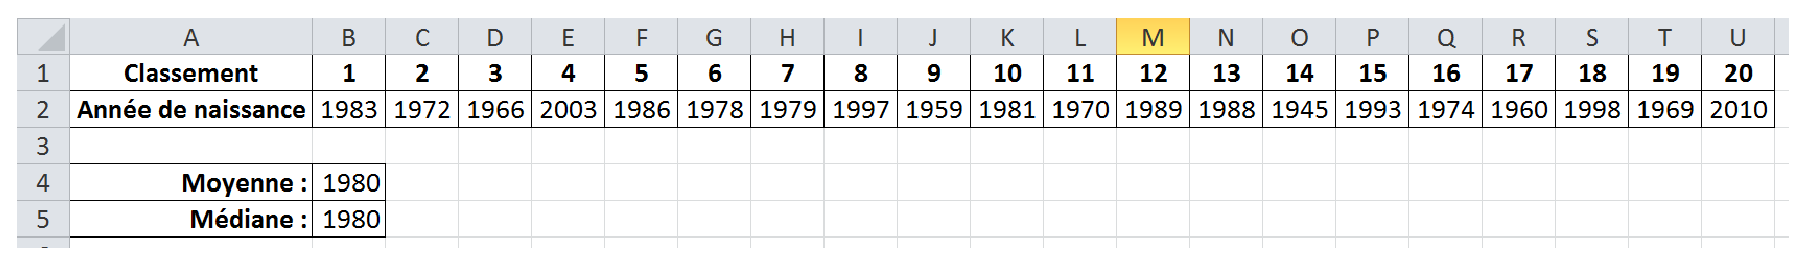
\includegraphics[scale=0.65]{stat.eps} 
\end{flushleft}

\initq \q La moyenne de la série a été calculée dans la cellule B4.\\
Quelle formule a été saisie dans la cellule B4 ?\\

\q Astrid remarque que la moyenne et la médiane de cette série sont égales.\\
Est-ce le cas pour n'importe quelle autre série statistique ? Expliquer votre réponse.\\

\textit{Rappel : La médiane d'une série statistique est le nombre qui partage cette série en deux groupes de même effectif.}\\






\end{document}
